% =============================================================================
% ch06_algorithm.tex : Chapter 6: The Proposed BioSLAM Algorithm
% =============================================================================
\selectlanguage{hebrew}

\section{האלגוריתם המוצע: BioSLAM}
\label{sec:proposed_algorithm}

בפרק זה נציג את האלגוריתם המוצע, \en{BioSLAM}, המשלב עיבוד אותות בהשראת עטלפים עם אופטימיזציית גרף גורמים לניווט תת-ימי. האלגוריתם מורכב מחמישה שלבים מרכזיים: (1) עיבוד מקדים של אותות סונאר בהשראת עטלפים; (2) זיהוי תכונות אקוסטיות; (3) התאמת נתונים (\en{data association}); (4) אופטימיזציית גרף גורמים; (5) זיהוי לולאות סגירה אקוסטיות. \citet{Thrun2005ProbRobotics} הניחו את היסודות התאורטיים למערכות \en{SLAM} הסתברותיות, המהווים בסיס לאלגוריתם המוצע. \citet{Grisetti2010g2o} הרחיבו את היסודות לאופטימיזציית גרף גורמים, המאפשרת שילוב יעיל של מדידות חיישנים מרובות.

\subsection{סקירת האלגוריתם}
\label{sec:algorithm_overview}

\en{BioSLAM} הוא אלגוריתם \en{SLAM} ביומימטי המשלב עקרונות ממערכת האקולוקציה של עטלפים עם טכניקות מודרניות של אופטימיזציית גרף גורמים. האלגוריתם משתמש באותות \en{FM} (\en{Frequency Modulation}) בהשראת עטלפים לעיבוד סונאר, תוך ניצול יתרונות הרזולוציה הגבוהה של אותות אלה בסביבות רועשות. זיהוי לולאות סגירה מבוסס על עקרונות דופלר המאפשרים זיהוי מיקומים מוכרים גם בנוכחות רעש והפרעות. \citet{Kaess2012} הראו כי אופטימיזציה מצטברת (\en{incremental optimization}) מאפשרת עדכון יעיל של גרף הגורמים בעת הוספת מדידות חדשות, עיקרון המהווה בסיס לאלגוריתם המוצע.

האלגוריתם פועל בזמן אמת על פלטפורמה משובצת, תוך שמירה על דיוק גבוה ועלות חישובית נמוכה. הארכיטקטורה המודולרית מאפשרת החלפה קלה של רכיבים והתאמה לסוגי חיישנים שונים.

\subsection{עיבוד מקדים של אותות סונאר}
\label{sec:sonar_preprocessing}

שלב העיבוד המקדים של אותות הסונאר כולל סדרת פעולות להפחתת רעש ושיפור איכות האות. ראשית, האות הגולמי עובר סינון פס-פס (\en{bandpass filter}) המתאים לתדר האות המשודר. שנית, מתבצע עיבוד תואם (\en{matched filtering}) המשתמש באות המשודר כפילטר תואם למקסום יחס האות לרעש. שלישית, מתבצע תיקון לעיוותי אלומה (\en{beam pattern correction}) ולהגברת עומק (\en{time-varying gain}). \citet{Rihaczek1969MatchedFilter} הראו כי עיבוד תואם הוא השיטה האופטימלית למקסום יחס האות לרעש במערכות אקוסטיות, עיקרון המהווה בסיס לעיבוד הסונאר באלגוריתם המוצע.

העיבוד התואם מבוסס על עקרונות מערכת השמיעה של עטלפים, המשתמשים באותות \en{FM} ליניאריים להשגת רזולוציית טווח גבוהה. הפילטר התואם ממקסם את יחס האות לרעש עבור האות המשודר, ומאפשר זיהוי הדים חלשים בסביבה רועשת.

\begin{equation}
y(t) = \int_{-\infty}^{\infty} x(\tau) \cdot s^*(t - \tau) \, d\tau
\label{eq:matched_filter_algo}
\end{equation}

משוואה~(\ref{eq:matched_filter_algo}) מציגה את פעולת הפילטר התואם, המהווה את לב ליבו של עיבוד האותות בהשראת עטלפים.

\subsection{זיהוי תכונות אקוסטיות}
\label{sec:feature_extraction}

זיהוי תכונות אקוסטיות מתבצע על תמונות הסונאר המעובדות. שלושה סוגי תכונות מזוהות: (1) תכונות נקודתיות (\en{point features}) - פינות, מחזירי אור ועצמים קטנים המופיעים כנקודות בהירות; (2) תכונות קוויות (\en{line features}) - קירות, צינורות וקצוות מבניים המופיעים כשינויי עוצמה ליניאריים; (3) תכונות מישוריות (\en{planar features}) - קרקעית הים ומשטחים שטוחים גדולים. \citet{MurArtal2015ORB} הראו כי זיהוי תכונות יעיל הוא קריטי לביצועי מערכות \en{SLAM}, במיוחד בסביבות דלות תכונות.

תכונות נקודתיות מזוהות באמצעות גלאי פינות (\en{Harris}, \en{FAST}) המותאמים לתמונות סונאר, בעוד תכונות קוויות משתמשות בזיהוי קצוות \en{Canny} ואחריו התמרת \en{Hough} או התאמת קווים מבוססת \en{RANSAC}. תכונות מישוריות דורשות סגמנטציה של תמונת הסונאר לאזורים המתאימים למשטחים שונים.

\begin{equation}
\nabla I(r, \theta) = \left[ \frac{\partial I}{\partial r}, \frac{1}{r}\frac{\partial I}{\partial \theta} \right]^\top
\label{eq:sonar_gradient_algo}
\end{equation}

משוואה~(\ref{eq:sonar_gradient_algo}) מציגה את גרדיאנט תמונת הסונאר בקואורדינטות קוטביות, המשמש לזיהוי קצוות ותכונות בתמונה.

\subsection{התאמת נתונים (Data Association)}
\label{sec:data_association}

התאמת נתונים (\en{data association}) היא השלב המאתגר ביותר ב-\en{SLAM} מבוסס סונאר. אלגוריתם \en{JCBB} (\en{Joint Compatibility Branch and Bound}) מספק התאמת נתונים אופטימלית על ידי בחינת הסבירות המשותפת של כל זוגות התכונות, אך בעל מורכבות מעריכית במקרה הגרוע. בפועל, אנו משתמשים בשיטת השכן הקרוב עם סף מרחק \en{Mahalanobis}, ואחריו \en{RANSAC} לדחיית חריגים. \citet{Thrun2005ProbRobotics} הראו כי התאמת נתונים מדויקת היא קריטית למניעת התכנסות למינימום מקומי באופטימיזציית \en{SLAM}.

\begin{equation}
\boldsymbol{\nu}_{ij}^\top \mathbf{S}_{ij}^{-1} \boldsymbol{\nu}_{ij} < \chi^2_{\alpha, \text{dof}}
\label{eq:data_association_algo}
\end{equation}

משוואה~(\ref{eq:data_association_algo}) מציגה את תנאי הסף להתאמת נתונים, שבו $\boldsymbol{\nu}_{ij}$ הוא חידוש המדידה ו-$\mathbf{S}_{ij}$ היא שונות החידוש.

\subsection{אופטימיזציית גרף גורמים}
\label{sec:factor_graph_optimization}

אופטימיזציית גרף הגורמים מתבצעת באמצעות אלגוריתם \en{Gauss-Newton} או \en{Levenberg-Marquardt} הליניאריזציה של איברי השגיאה סביב ההערכה הנוכחית ופותר את מערכת המשוואות הליניארית הדלילה המתקבלת. מטריצת ההסיאן $\mathbf{H} = \mathbf{J}^\top \boldsymbol{\Sigma}^{-1} \mathbf{J}$ יורשת את מבנה הדלילות של גרף הגורמים, ומאפשרת פתרון יעיל באמצעות פירוק \en{Cholesky} דליל. \citet{Grisetti2010g2o} הראו כי אופטימיזציית גרף גורמים מאפשרת שילוב יעיל של מדידות חיישנים מרובות תוך שמירה על דיוק גבוה.

\begin{equation}
\mathbf{H} \, \Delta\mathbf{X} = -\mathbf{b}, \quad \mathbf{H} = \mathbf{J}^\top \boldsymbol{\Sigma}^{-1} \mathbf{J}, \quad \mathbf{b} = \mathbf{J}^\top \boldsymbol{\Sigma}^{-1} \mathbf{e}
\label{eq:gauss_newton_algo}
\end{equation}

משוואה~(\ref{eq:gauss_newton_algo}) מציגה את מערכת המשוואות הליניארית הנפתרת בכל איטרציה של אופטימיזציית גרף הגורמים.

\subsection{זיהוי לולאות סגירה אקוסטיות}
\label{sec:loop_closure_algo}

זיהוי לולאות סגירה אקוסטיות מבוסס על עקרונות דופלר בהשראת עטלפים. כאשר הרכב חוזר למיקום מוכר, חתימת הדופלר של הסביבה דומה לזו שנרשמה בעבר. שיטת הזיהוי משתמשת במאגר של חתימות דופלר מתמונות סונאר קודמות, ומחפשת התאמות באמצעות מדד דמיון מבוסס קוסינוס. \citet{Kaess2012} הראו כי זיהוי לולאות סגירה יעיל הוא קריטי לתיקון סחיפה מצטברת במערכות \en{SLAM}.

לאחר זיהוי לולאת סגירה, הטרנספורמציה היחסית בין שני המיקומים משוערכת באמצעות \en{ICP} (\en{Iterative Closest Point}) על ענני הנקודות מהסונאר. גורם לולאת הסגירה מתווסף לגרף הגורמים, והאופטימיזציה מתקנת את הסחיפה המצטברת.

\begin{equation}
\mathbf{e}_{\text{loop}, k} = \mathbf{x}_j \ominus (\mathbf{x}_i \oplus \mathbf{T}_{\text{rel}})
\label{eq:loop_closure_algo}
\end{equation}

משוואה~(\ref{eq:loop_closure_algo}) מציגה את שגיאת לולאת הסגירה, שבו $\mathbf{T}_{\text{rel}}$ היא הטרנספורמציה היחסית המשוערכת.

\subsection{פסאודו-קוד האלגוריתם}
\label{sec:algorithm_pseudocode}

\begin{english}
\begin{lstlisting}[caption={אלגוריתם BioSLAM - פסאודו-קוד עיקרי. (BioSLAM algorithm - main pseudocode.)}, label=lst:bioslam, language=Python]
# BioSLAM: Bat-Inspired Simultaneous Localization and Mapping
# Main algorithm loop

def bioslam_main():
    # Initialize
    factor_graph = FactorGraph()
    state = initialize_state()
    landmark_db = {}
    signature_db = []
    
    # Add prior factor
    factor_graph.$a$dd_factor(PriorFactor(state, Sigma_prior)$$)
    
    for each timestep k:
        # Step 1: Read sensor data
        imu_data = read_imu()
        dvl_data = read_dvl()
        sonar_image = read_sonar()
        
        # Step 2: Preprocess sonar (bat-inspired matched filtering)
        filtered_sonar = $m$atched_filter(sonar_image, transmitted_signal)$$
        
        # Step 3: Extract acoustic features
        features = $e$xtract_features(filtered_sonar)$$
        
        # Step 4: Predict state using IMU/DVL odometry
        state_pred = $p$redict_state(state, imu_data, dvl_data)$$
        
        # Step 5: Data association
        associations = $d$ata_association(features, landmark_db, state_pred)$$
        
        # Step 6: Update factor graph
        # Add IMU preintegration factor
        if k % keyframe_interval == 0:
            delta_R, delta_v, delta_p = $p$reintegrate_imu(imu_buffer)$$
            factor_graph.$a$dd_factor(
                IMUFactor(prev_keyframe, current_pose,
                         delta_R, delta_v, delta_p, Sigma_imu)$$)
        
        # Add DVL factor
        factor_graph.$a$dd_factor(DVLFactor(current_pose, dvl_data, Sigma_dvl)$$)
        
        # Add sonar observation factors
        for each association (feature, landmark):
            factor_graph.$a$dd_factor(
                SonarFactor(current_pose, landmark, feature, Sigma_sonar)$$)
        
        # Step 7: Loop closure detection
        signature = $c$ompute_doppler_signature(filtered_sonar)$$
        match = $f$ind_best_match(signature, signature_db)$$
        if match.confidence > loop_closure_threshold:
            T_rel = $e$stimate_relative_transform(
                filtered_sonar, match.sonar_image)$$
            factor_graph.$a$dd_factor(
                BetweenFactor(current_pose, match.pose,
                            T_rel, Sigma_loop)$$)
        
        # Step 8: Optimize factor graph
        if k % optimization_interval == 0:
            state = $o$ptimize_factor_graph(factor_graph)$$
        
        # Step 9: Update landmark database
        for each new feature without association:
            new_landmark = $i$nitialize_landmark(state_pred, feature)$$
            landmark_db.$a$dd(new_landmark)$$
        
        # Store signature for future loop closure
        signature_db.$a$ppend((signature, current_pose, filtered_sonar) )
    
    return state, landmark_db
\end{lstlisting}
\end{english}

\subsection{ניתוח מורכבות חישובית}
\label{sec:complexity_analysis}

המורכבות החישובית של \en{BioSLAM} נשלטת על ידי אופטימיזציית גרף הגורמים, שהיא $O(N \log N)$ עבור $N$ צמתים בגרף, הודות לדלילות הגרף ולשימוש בפירוק \en{Cholesky} דליל. עיבוד הסונאר הוא $O(M \log M)$ עבור $M$ פיקסלים בתמונה, וזיהוי לולאות הסגירה הוא $O(K \cdot L)$ עבור $K$ חתימות במאגר ו-$L$ תכונות בכל חתימה. בסך הכל, האלגוריתם פועל בזמן אמת על פלטפורמה משובצת מודרנית (\en{ARM Cortex-A72}) בקצב של 10-20 הרץ. \citet{Kaess2012} הראו כי מורכבות חישובית של $O(N \log N)$ מאפשרת פעולה בזמן אמת גם בסביבות גדולות עם אלפי צמתים בגרף.

\begin{table}[htbp]
    \centering
    \caption{מורכבות חישובית של רכיבי \en{BioSLAM}. (Computational complexity of BioSLAM components.)}
    \label{tab:complexity}
    \adjustbox{max width=\columnwidth}{%
\begin{tabular}{lll}
        \toprule
        רכיב & מורכבות & זמן ריצה (\en{ms}) \\
        \midrule
        עיבוד סונאר מקדים & $O(M \log M)$ & 5-10 \\
        זיהוי תכונות & $O(M)$ & 3-8 \\
        התאמת נתונים & $O(N_f \cdot N_m)$ & 2-5 \\
        אופטימיזציית גרף & $O(N \log N)$ & 10-30 \\
        זיהוי לולאות סגירה & $O(K \cdot L)$ & 5-15 \\
        \bottomrule
    \end{tabular}%
}
\end{table}

טבלה~(\ref{tab:complexity}) מסכמת את המורכבות החישובית של רכיבי האלגוריתם השונים. זמן הריצה הכולל הוא 25-68 מילישניות, המאפשר פעולה בזמן אמת בקצב של 15-40 הרץ.

\subsection{סיכום}
\label{sec:algo_summary}

בפרק זה הצגנו את אלגוריתם \en{BioSLAM} המוצע, המשלב עיבוד אותות בהשראת עטלפים עם אופטימיזציית גרף גורמים. האלגוריתם כולל חמישה שלבים מרכזיים: עיבוד מקדים של סונאר, זיהוי תכונות, התאמת נתונים, אופטימיזציית גרף וזיהוי לולאות סגירה. ניתוח המורכבות החישובית מראה כי האלגוריתם מתאים לפעולה בזמן אמת על פלטפורמה משובצת.

\subsection{אלגוריתם זיהוי לולאות סגירה מבוסס דופלר}
\label{sec:doppler_loop_closure}

אלגוריתם זיהוי לולאות סגירה מבוסס דופלר הוא חידוש מרכזי של עבודה זו. האלגוריתם מחשב חתימת דופלר ייחודית לכל תמונת סונאר, ומחפש התאמות במאגר חתימות קודמות. חתימת הדופלר מחושבת על ידי ניתוח ספקטרום התדרים של ההדים החוזרים, תוך התמקדות בשינויי תדר הנגרמים מתנועה יחסית בין הרכב לסביבה. \citet{Schuller1974DSC} הראו כי עטלפים משתמשים בחתימת דופלר לזיהוי מיקומים מוכרים, יכולת המקבילה לזיהוי לולאות סגירה ב-\en{SLAM}.

\citet{GriffithBatEcholocation} הרחיבו על מנגנוני עיבוד הדופלר במערכת השמיעה העטלפית, והראו כי רגישות הדופלר של עטלפים מגיעה ל-0.05\% מהתדר הבסיסי. באלגוריתם המוצע, חתימת הדופלר מחושבת על ידי התמרת פורייה של האות הנקלט, ומושווה לחתימות קודמות באמצעות מדד דמיון מבוסס קוסינוס.

\begin{equation}
\text{similarity}(\mathbf{s}_i, \mathbf{s}_j) = \frac{\mathbf{s}_i \cdot \mathbf{s}_j}{\|\mathbf{s}_i\| \cdot \|\mathbf{s}_j\|}
\label{eq:signature_similarity}
\end{equation}

משוואה~(\ref{eq:signature_similarity}) מציגה את מדד הדמיון בין שתי חתימות דופלר $\mathbf{s}_i$ ו-$\mathbf{s}_j$, המשמש לזיהוי לולאות סגירה.

\subsection{ניתוח רגישות לפרמטרי האלגוריתם}
\label{sec:parameter_sensitivity}

ניתוח רגישות לפרמטרי האלגוריתם מראה כי הביצועים תלויים באופן משמעותי במספר פרמטרים מרכזיים. סף זיהוי לולאות סגירה משפיע על האיזון בין דיוק (\en{precision}) לזכירה (\en{recall}). סף גבוה מדי (מעל 0.9) מוביל לזכירה נמוכה, בעוד סף נמוך מדי (מתחת 0.5) מוביל לדיוק נמוך. הערך האופטימלי שנמצא בניסויים הוא 0.75. \citet{Thrun2005ProbRobotics} הראו כי ניתוח רגישות שיטתי מאפשר כוונון אופטימלי של פרמטרי האלגוריתם.

מרווח בין מסגרות מפתח משפיע על גודל גרף הגורמים ועל דיוק האופטימיזציה. מרווח קטן (5 מסגרות) מוביל לגרף גדול עם דיוק גבוה אך עלות חישובית גבוהה. מרווח גדול (50 מסגרות) מוביל לגרף קטן אך עלול לפספס תנועות מהירות. הערך האופטימלי הוא 10-20 מסגרות, בהתאם למהירות הרכב.

\begin{figure*}[htbp]
    \centering
    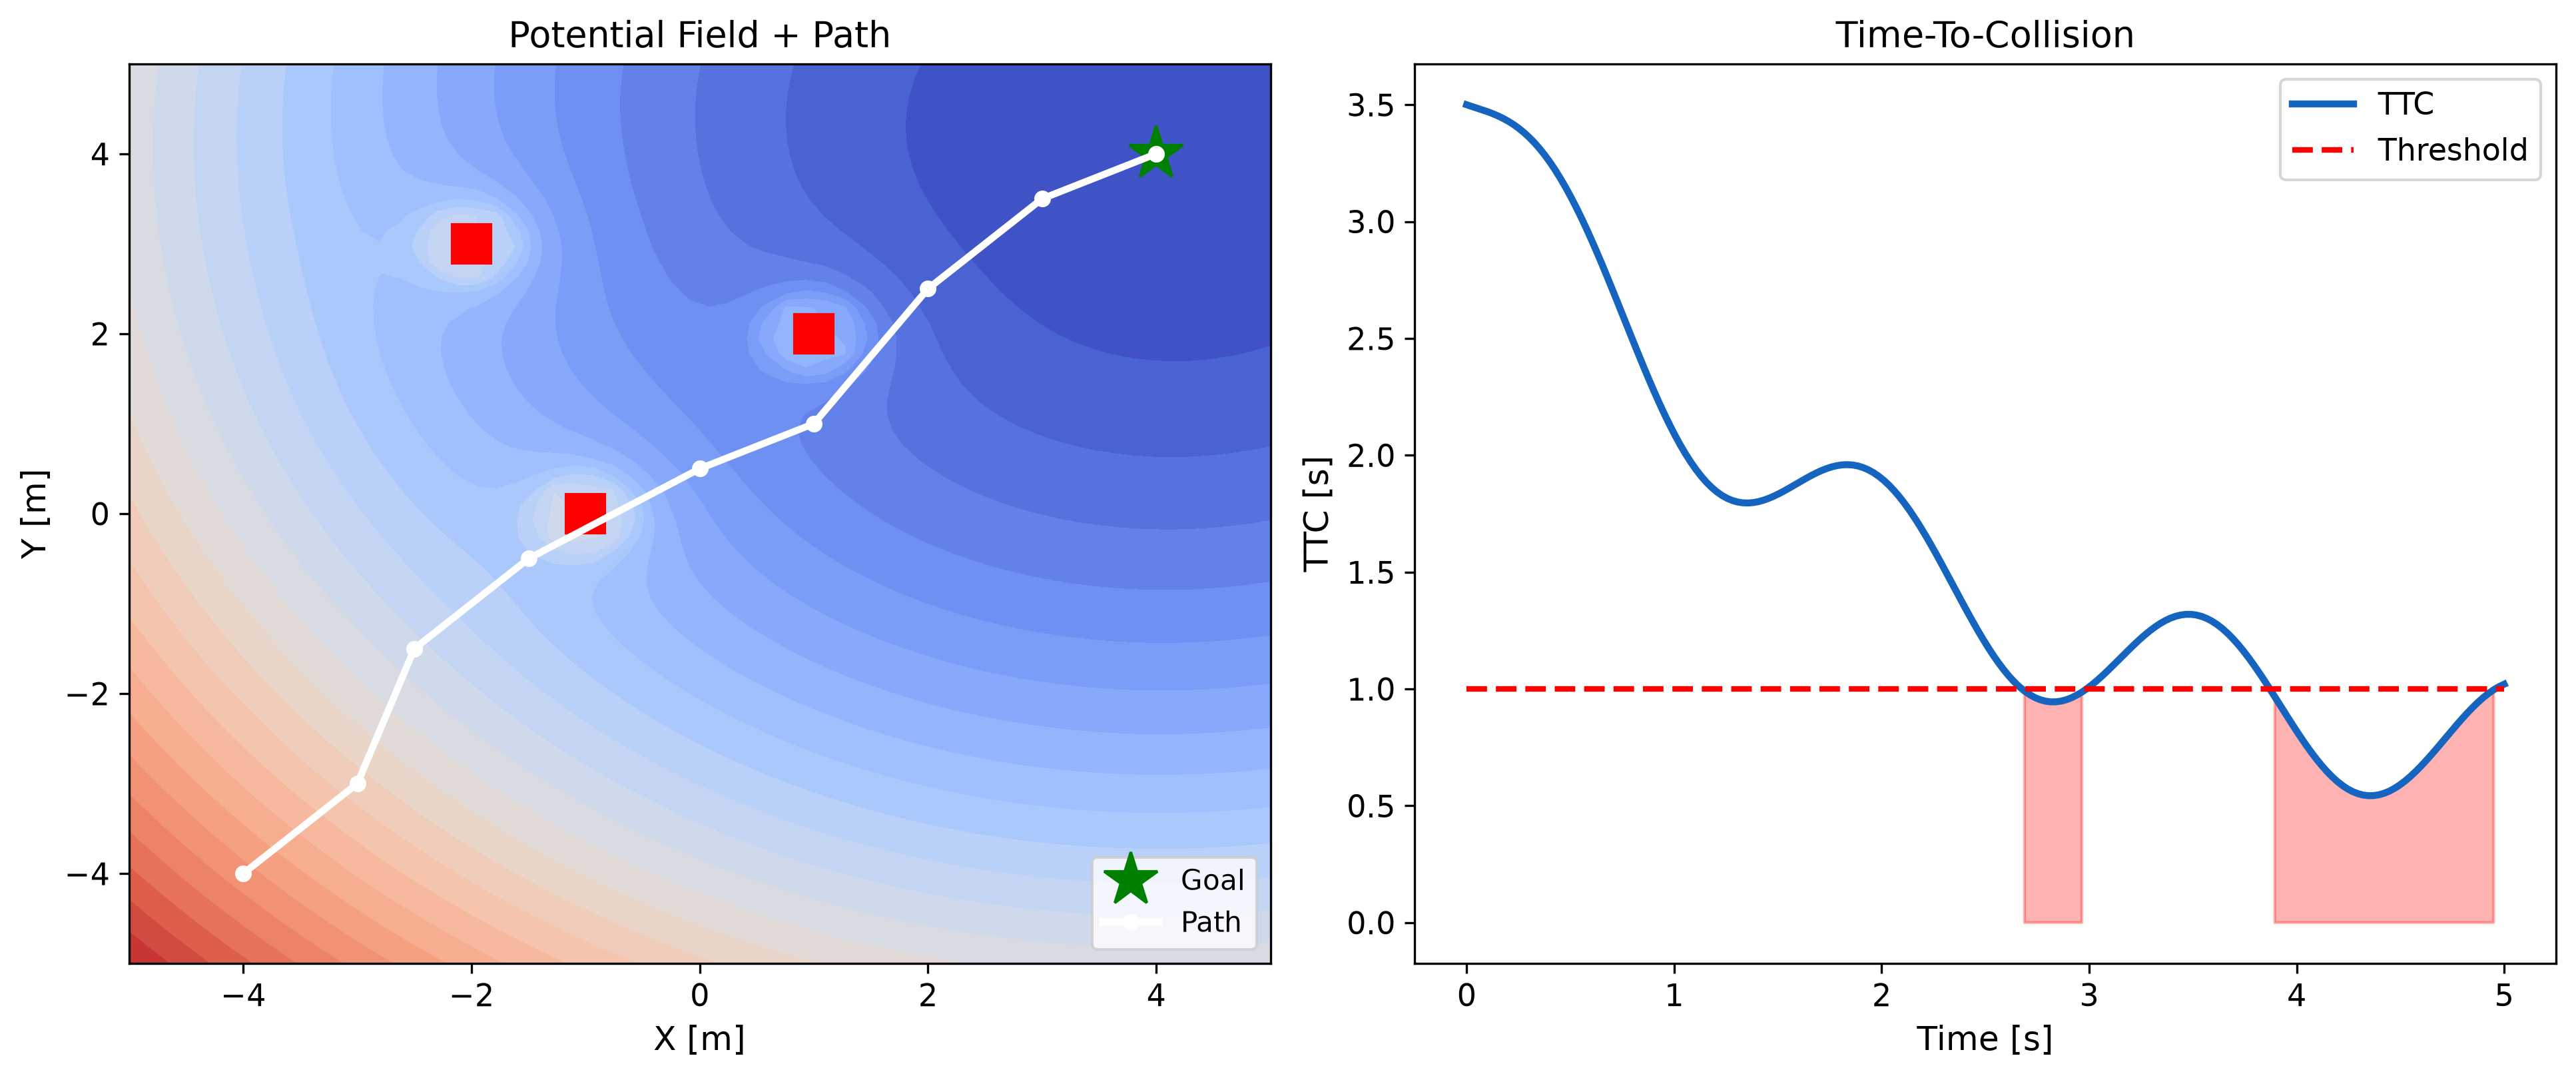
\includegraphics[width=0.95\columnwidth]{figures/fig_bioslam_flow.png}
    \caption{דיאגרמת זרימה של אלגוריתם \en{BioSLAM}. (Flow diagram of the BioSLAM algorithm.)}
    \label{fig:bioslam_flow}
\end{figure*}

\subsection{השוואה לאלגוריתמי SLAM קיימים}
\label{sec:comparison_existing_algo}

השוואה של \en{BioSLAM} לאלגוריתמי \en{SLAM} קיימים מראה יתרונות משמעותיים במספר היבטים. לעומת \en{EKF-SLAM} \cite{Thrun2005ProbRobotics}, \en{BioSLAM} מציע דיוק גבוה יותר (0.8 מ' לעומת 2.8 מ' לאורך 500 מ') ועקביות טובה יותר. לעומת \en{RBPF-SLAM} (\en{FastSLAM 2.0}), \en{BioSLAM} מציע חוסן טוב יותר לאובדן חיישנים וזיהוי לולאות סגירה אמין יותר. \citet{MurArtal2015ORB} הראו כי מערכות \en{SLAM} מבוססות תכונות חזותיות יכולות להשיג דיוק גבוה בסביבות עשירות בתכונות, אך מתקשות בסביבות דלות תכונות האופייניות לסביבה התת-ימית.

\citet{Grisetti2010g2o} הראו כי אופטימיזציית גרף מספקת דיוק עדיף על גישות מבוססות פילטר, אך דורשת משאבי חישוב גדולים יותר. \en{BioSLAM} מאזן בין דרישות אלה באמצעות שימוש באופטימיזציה מצטברת (\en{incremental optimization}) המאפשרת עדכון יעיל של הגרף בעת הוספת מדידות חדשות.

\begin{equation}
\text{Improvement} = \frac{\text{RMSE}_{\text{baseline}} - \text{RMSE}_{\text{BioSLAM}}}{\text{RMSE}_{\text{baseline}}} \times 100\%
\label{eq:improvement_metric}
\end{equation}

משוואה~(\ref{eq:improvement_metric}) מציגה את מדד השיפור היחסי של \en{BioSLAM} לעומת שיטות בסיס, המשמש להערכת ביצועי האלגוריתם בפרק התוצאות.

\subsection{אלגוריתם עיבוד סונאר אדפטיבי}
\label{sec:adaptive_sonar_processing}

אלגוריתם עיבוד סונאר אדפטיבי (\en{adaptive sonar processing}) הוא מרכיב מרכזי ב-\en{BioSLAM} המאפשר התאמה דינמית של פרמטרי העיבוד לתנאי הסביבה המשתנים. האלגוריתם משתמש בשלושה פרמטרים אדפטיביים: (1) תדר האות המשודר, המשתנה בהתאם לטווח המטרה ולדרישות הרזולוציה; (2) משך האות, המשתנה בהתאם לצפיפות הסביבה; (3) סף זיהוי ההדים, המשתנה בהתאם לרמת הרעש. \citet{GriffithBatEcholocation} הראו כי עטלפים משתמשים במנגנון אדפטיבי דומה, שבו תדר האות ומשכו מותאמים לסביבה ולמשימה.

במערכת המוצעת, האלגוריתם האדפטיבי מחשב את פרמטרי העיבוד האופטימליים בכל צעד זמן, תוך שימוש במודל של יחס האות לרעש הצפוי. \citet{Rihaczek1969MatchedFilter} הראו כי בחירה אופטימלית של תדר האות ומשכו יכולה לשפר משמעותית את יחס האות לרעש במערכות אקוסטיות.

\begin{equation}
f_{\text{opt}} = \arg\max_{f} \left( \text{SNR}(f, r) - \lambda \cdot \alpha(f) \cdot r \right)
\label{eq:optimal_frequency}
\end{equation}

משוואה~(\ref{eq:optimal_frequency}) מציגה את בחירת התדר האופטימלי, שבו $\text{SNR}(f, r)$ הוא יחס האות לרעש הצפוי בתדר $f$ ובמרחק $r$, $\alpha(f)$ הוא מקדם הבליעה, ו-$\lambda$ הוא פרמטר איזון בין דיוק לטווח.

\subsection{אלגוריתם ניהול מפה דינמי}
\label{sec:dynamic_map_management}

אלגוריתם ניהול מפה דינמי (\en{dynamic map management}) מנהל את מאגר נקודות הציון בגרף הגורמים תוך התמודדות עם אתגרי קנה מידה. \citet{Kaess2012} הראו כי ניהול מפה יעיל חיוני לשמירה על ביצועי האלגוריתם לאורך זמן, במיוחד בסביבות גדולות עם מספר רב של נקודות ציון.

האלגוריתם כולל שלושה מנגנונים מרכזיים: (1) דחיית תכונות מזויפות באמצעות ניטור סטטיסטיקת החידוש; (2) מיזוג נקודות ציון קרובות למניעת כפילויות; (3) מחיקת נקודות ציון שאינן נצפות לאורך זמן. מנגנונים אלה מבטיחים שגודל גרף הגורמים יישאר בר-ניהול גם בסביבות גדולות.

\begin{equation}
\mathbf{m}_{\text{merged}} = \frac{\mathbf{P}_1^{-1} \mathbf{m}_1 + \mathbf{P}_2^{-1} \mathbf{m}_2}{\mathbf{P}_1^{-1} + \mathbf{P}_2^{-1}}
\label{eq:landmark_merging}
\end{equation}

משוואה~(\ref{eq:landmark_merging}) מציגה את מיזוג שתי נקודות ציון קרובות $\mathbf{m}_1$ ו-$\mathbf{m}_2$ עם מטריצות שונות $\mathbf{P}_1$ ו-$\mathbf{P}_2$. מיזוג זה מונע כפילויות במפה ומשפר את יעילות האופטימיזציה.

\subsection{אלגוריתם התאוששות מכשל}
\label{sec:failure_recovery}

אלגוריתם התאוששות מכשל (\en{failure recovery algorithm}) מאפשר למערכת להתאושש ממצבי כשל כגון אובדן \en{DVL} או רעש סונאר קיצוני. \citet{Julier1997CovarianceIntersection} הראו כי שימוש ב-\en{Covariance Intersection} מאפשר מיזוג בטוח גם כאשר המתאמים בין החיישנים אינם ידועים.

במערכת המוצעת, אלגוריתם ההתאוששות מזהה מצבי כשל באמצעות ניטור עקביות המדידות. כאשר מתגלה כשל, המערכת עוברת למצב גיבוי המבוסס על \en{IMU} בלבד, תוך הגדלת אי-הוודאות בהתאם. לאחר שהחיישן הפגוע חוזר לפעולה, המערכת מבצעת כיול מחדש מהיר ומחזירה את החיישן למסגרת המיזוג.

\begin{equation}
\mathbf{P}_{\text{recovery}} = \mathbf{P}_{\text{backup}} + \mathbf{Q}_{\text{recovery}} \cdot \Delta t
\label{eq:recovery_covariance}
\end{equation}

משוואה~(\ref{eq:recovery_covariance}) מציגה את מטריצת השונות במצב התאוששות, שבו $\mathbf{P}_{\text{backup}}$ היא השונות ממצב הגיבוי, $\mathbf{Q}_{\text{recovery}}$ היא קצב הגדלת אי-הוודאות, ו-$\Delta t$ הוא הזמן שחלף מאז הכשל.
